\section{Duration in time units}
\label{sec-change-location}

\textbf{Created by:} Arkopaul Sarkar \\
\textbf{Modified by:} Arkopaul Sarkar \\

\subsection*{Scenario Objective}

This scenario demonstrates how to represent time durations of time intervals. Duration values can be measured in different time units, such as years, hours, and ticks. In the following, we present the patterns for asserting duration values in standard and custom units.   

\subsection*{General Pattern Description}

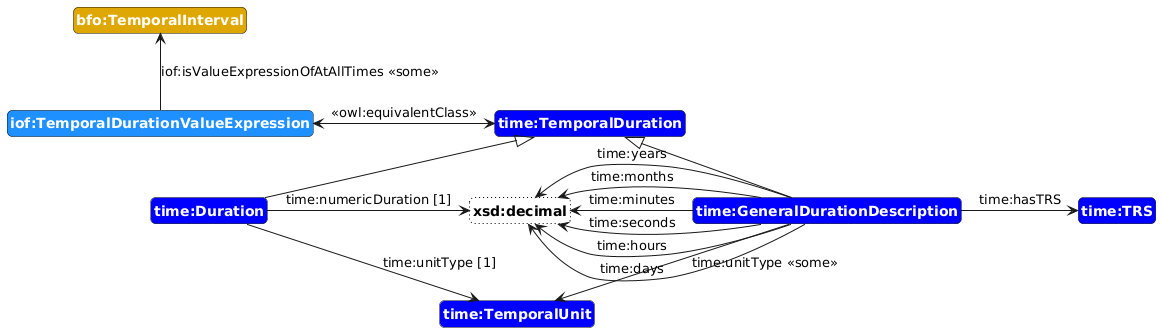
\includegraphics[scale=0.36]{scenarios/time-duration/image/time-duration.png}

The duration of a temporal interval can be expressed by associating different instances of \\ \cname{iof}{TemporalDurationValueExpression} or some subtype of the OWL-Time class \cname{time}{TemporalDuration} to the instance of \cname{bfo}{TemporalInterval} using \opname{iof}{isValueExpressionOfAtAllTimes}, as they are equivalent classes. An instance of \cname{time}{DurationDescription}, which is a subclass of \cname{time}{TemporalDuration}, provides several data properties to assert the duration value in various units used in Gregorian Calendar, e.g., \dpname{time}{years}, \dpname{time}{months}, and \dpname{time}{minutes}. Alternatively, a numeric value and corresponding duration type can be asserted using the instance of \cname{time}{Duration}. A custom duration description class can be defined by extending the \cname{time}{GeneralDurationDescription} class with an appropriate temporal reference system. 

\subsubsection*{Use Case: Duration of OntoCommons project} 
OntoCommons project started on Wednesday, 1 September 2021 and ended on Saturday, 9 November 2024. It ran for 1165 days from the start to the end date, not including the end date.

The duration of the temporal interval (\iname{ns1}{oc-project-interval}), that the project (\iname{ns1}{ontocommons-project}) ran for, can be expressed in typical duration units from Gregorian calendar, e.g., year, month, day, hour, minute, and second, using OWL Time classes. OWL Time also provides mechanisms for creating custom duration descriptions. 

\subsubsection*{Use-Case Pattern Description}

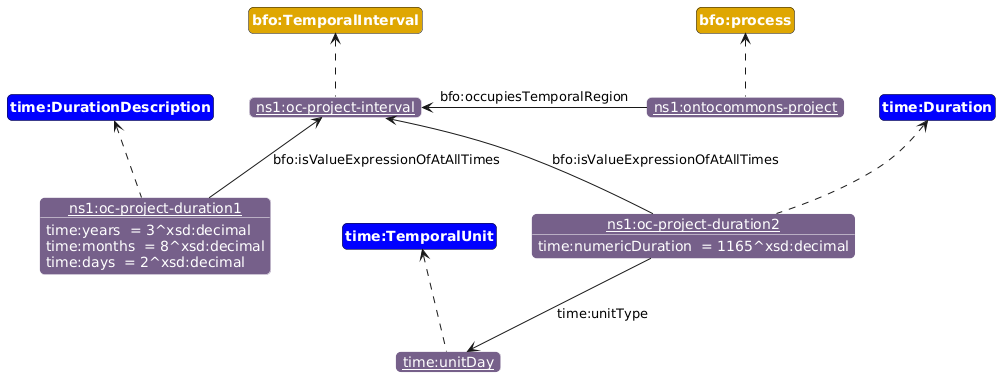
\includegraphics[scale=0.40]{scenarios/time-duration/image/uc1-time-duration.png}

The duration value can be expressed by linking an instance of \cname{time}{DurationDescription} or \cname{time}{Duration}. \cname{}{DurationDescription} provides dedicated data properties in various units, allowing users to express the duration value in mixed units, e.g., the project duration is 3 years 8 months and 2 days. \cname{time}{Duration} allows expression of the duration value in a single unit (various common unit instances are already provided by OWL Time), e.g., 1165 days.

\paragraph{Using custom clock time format \\}

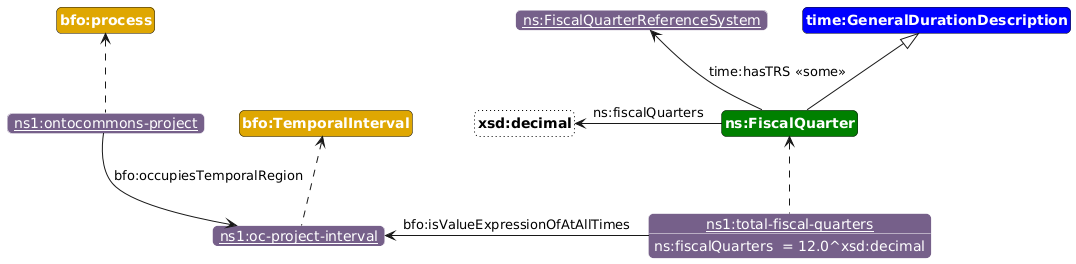
\includegraphics[scale=0.38]{scenarios/time-duration/image/uc2-custom-duration.png}

In the above pattern the launch date is expressed in `Fiscal Quarters'. The new duration description class \cname{}{DurationDescriptionInFiscalQuater}, extended from \cname{time}{GeneralDurationDescription}, with the restriction that the number of fiscal quarter can be asserted in decimal using only \dpname{ns}{fiscalQuarters} data property. The example does not provide details of \iname{}{FiscalQuarterReferenceSystem}, which is a \cname{time}{TemporalReferenceSystem}, and may refer to a suitable description of `fiscal quarter'. 


\subsubsection*{Data Mapping Description}

\begin{verbatim}
INSERT DATA {
    ns1:ontocommons-project a bfo:Process ;
                             bfo:occupiesTemporalRegion ns1:oc-project-interval .

    ns1:oc-project-interval a bfo:TemporalInterval .

    ns1:oc-project-duration1 a time:DurationDescription ;
                              iof:isValueExpressionOfAtAllTimes ns1:oc-project-interval ;
                              time:years "3"^^xsd:decimal ;
                              time:months "8"^^xsd:decimal ;
                              time:days "2"^^xsd:decimal .

    ns1:oc-project-duration2 a time:Duration ;
                              iof:isValueExpressionOfAtAllTimes ns1:oc-project-interval ;
                              time:numericDuration "1165"^^xsd:decimal ;
                              time:unitType time:unitDay .

    ns1:oc-project-duration3 a ns:FiscalQuarter ;
                              iof:isValueExpressionOfAtAllTimes ns1:oc-project-interval ;
                              ns:fiscalQuarters "12"^^xsd:decimal .
}
\end{verbatim}

The \cname{ns}{DurationDescriptionInFiscalQuarter} class has a temporal reference system as \\ \cname{ns}{FiscalQuarterReferenceSystem}, which refers to the specification of fiscal quarter duration format. The class restrict the usage of other data properties from \cname{time}{GeneralDurationDescription} and allows exactly one decimal value to be linked with data property \dpname{ns}{fiscalQuarters}

\begin{verbatim}
:DurationDescriptionInFiscalQuarter rdf:type owl:Class ;
    rdfs:subClassOf 
        <http://www.w3.org/2006/time#DurationDescription> ,
        
        [ rdf:type owl:Restriction ;
          owl:onProperty <http://www.w3.org/2006/time#hasTRS> ;
          owl:allValuesFrom :FiscalQuarterReferenceSystem
        ] ,
        
        [ rdf:type owl:Restriction ;
          owl:onProperty :fiscalQuarters ;
          owl:qualifiedCardinality "1"^^xsd:nonNegativeInteger ;
          owl:onDataRange xsd:decimal
        ] ,
        
        [ rdf:type owl:Restriction ;
          owl:onProperty <http://www.w3.org/2006/time#days> ;
          owl:cardinality "0"^^xsd:nonNegativeInteger
        ] ,
        
        [ rdf:type owl:Restriction ;
          owl:onProperty <http://www.w3.org/2006/time#hours> ;
          owl:cardinality "0"^^xsd:nonNegativeInteger
        ] ,
        
        [ rdf:type owl:Restriction ;
          owl:onProperty <http://www.w3.org/2006/time#minutes> ;
          owl:cardinality "0"^^xsd:nonNegativeInteger
        ] ,
        
        [ rdf:type owl:Restriction ;
          owl:onProperty <http://www.w3.org/2006/time#months> ;
          owl:cardinality "0"^^xsd:nonNegativeInteger
        ] ,
        
        [ rdf:type owl:Restriction ;
          owl:onProperty <http://www.w3.org/2006/time#seconds> ;
          owl:cardinality "0"^^xsd:nonNegativeInteger
        ] ,
        
        [ rdf:type owl:Restriction ;
          owl:onProperty <http://www.w3.org/2006/time#weeks> ;
          owl:cardinality "0"^^xsd:nonNegativeInteger
        ] ,
        
        [ rdf:type owl:Restriction ;
          owl:onProperty <http://www.w3.org/2006/time#years> ;
          owl:cardinality "0"^^xsd:nonNegativeInteger
        ] .

:FiscalQuarterReferenceSystem rdf:type owl:Class ;
    rdfs:subClassOf <http://www.w3.org/2006/time#TRS> .

\end{verbatim}


\subsubsection*{Data Validation}

